\documentclass{article}
\usepackage[utf8]{inputenc}
\usepackage{amsmath}
\usepackage{amsfonts}
\usepackage{amssymb}
\usepackage{listings} % Para resaltar la sintaxis del código
\usepackage{graphicx}
\usepackage{tcolorbox}
\usepackage{color}
\usepackage[left=2cm,right=2cm,top=3.5cm,bottom=3.5cm]{geometry}

\definecolor{codegreen}{rgb}{0,0.6,0}
\definecolor{codegray}{rgb}{0.5,0.5,0.5}
\definecolor{codepurple}{rgb}{0.58,0,0.82}
\definecolor{backcolour}{rgb}{0.95,0.95,0.92}

\lstdefinestyle{mystyle}{
    backgroundcolor=\color{backcolour},   
    commentstyle=\color{codegreen},
    keywordstyle=\color{magenta},
    numberstyle=\tiny\color{codegray},
    stringstyle=\color{codepurple},
    basicstyle=\ttfamily\footnotesize,
    breakatwhitespace=false,         
    breaklines=true,                 
    captionpos=b,                    
    keepspaces=true,                 
    numbers=left,                    
    numbersep=5pt,                  
    showspaces=false,                
    showstringspaces=false,
    showtabs=false,                  
    tabsize=2
}

\lstset{style=mystyle}


% Portada
\title{\Huge \textbf{Práctica 1. Administración básica de un
servidor}}
\author{Diego Esclarín Fernández}
\date{\today}


\begin{document}

\begin{titlepage}
    \maketitle
    \ 
    \begin{figure}[h]
        \centering
        
\includegraphics[width=0.6\textwidth]{Logo_URJC.png}
        \label{fig:ejemplo}
    \end{figure}
\end{titlepage}


% Contenido del documento
\section{Introducción}
Los objetivos de esta práctica son:
\begin{itemize}
  \item Poner en marcha un servidor Linux accesible.
  \item Securizarlo y programar un script de mantenimiento.
  \item Instalar y mantener levantada una API-Rest en Python.
\end{itemize}

\



% Segundo punto
\section{Paso a paso}
\subsection{Administración básica de un servidor}
\begin{itemize}
  \item Crear una instancia de EC2 en AWS (Amazon Elastic Compute Cloud) utilizando la consola de AWS.
  \item Conectar a la instancia utilizando SSH desde tu terminal o cliente SSH favorito.
\end{itemize}

% Conexión SSH
\subsubsection{Conexión SSH:}
\begin{enumerate}
  \item Entrar en \textit{Visual Studio Code} y conectarse a la máquina virtual.
  \item Moverse hasta la carpeta de la clave de entrada al servidor.
  \item Ejecutar el comando: \texttt{chmod 400 "Nombre\_de\_la\_clave.pem"} en terminal.
  \item Ir a ``conectar" en AWS al seleccionar la instancia y copiar el ejemplo y cambiar el nombre de la llave.
\end{enumerate}

\

% Configuración inicial
\subsection{Puesta en marcha de un servidor Linux accesible}
\begin{itemize}
  \item Elegir una imagen de sistema operativo Linux compatible al crear la instancia EC2.
\end{itemize}

\begin{figure}[ht]
    \centering
    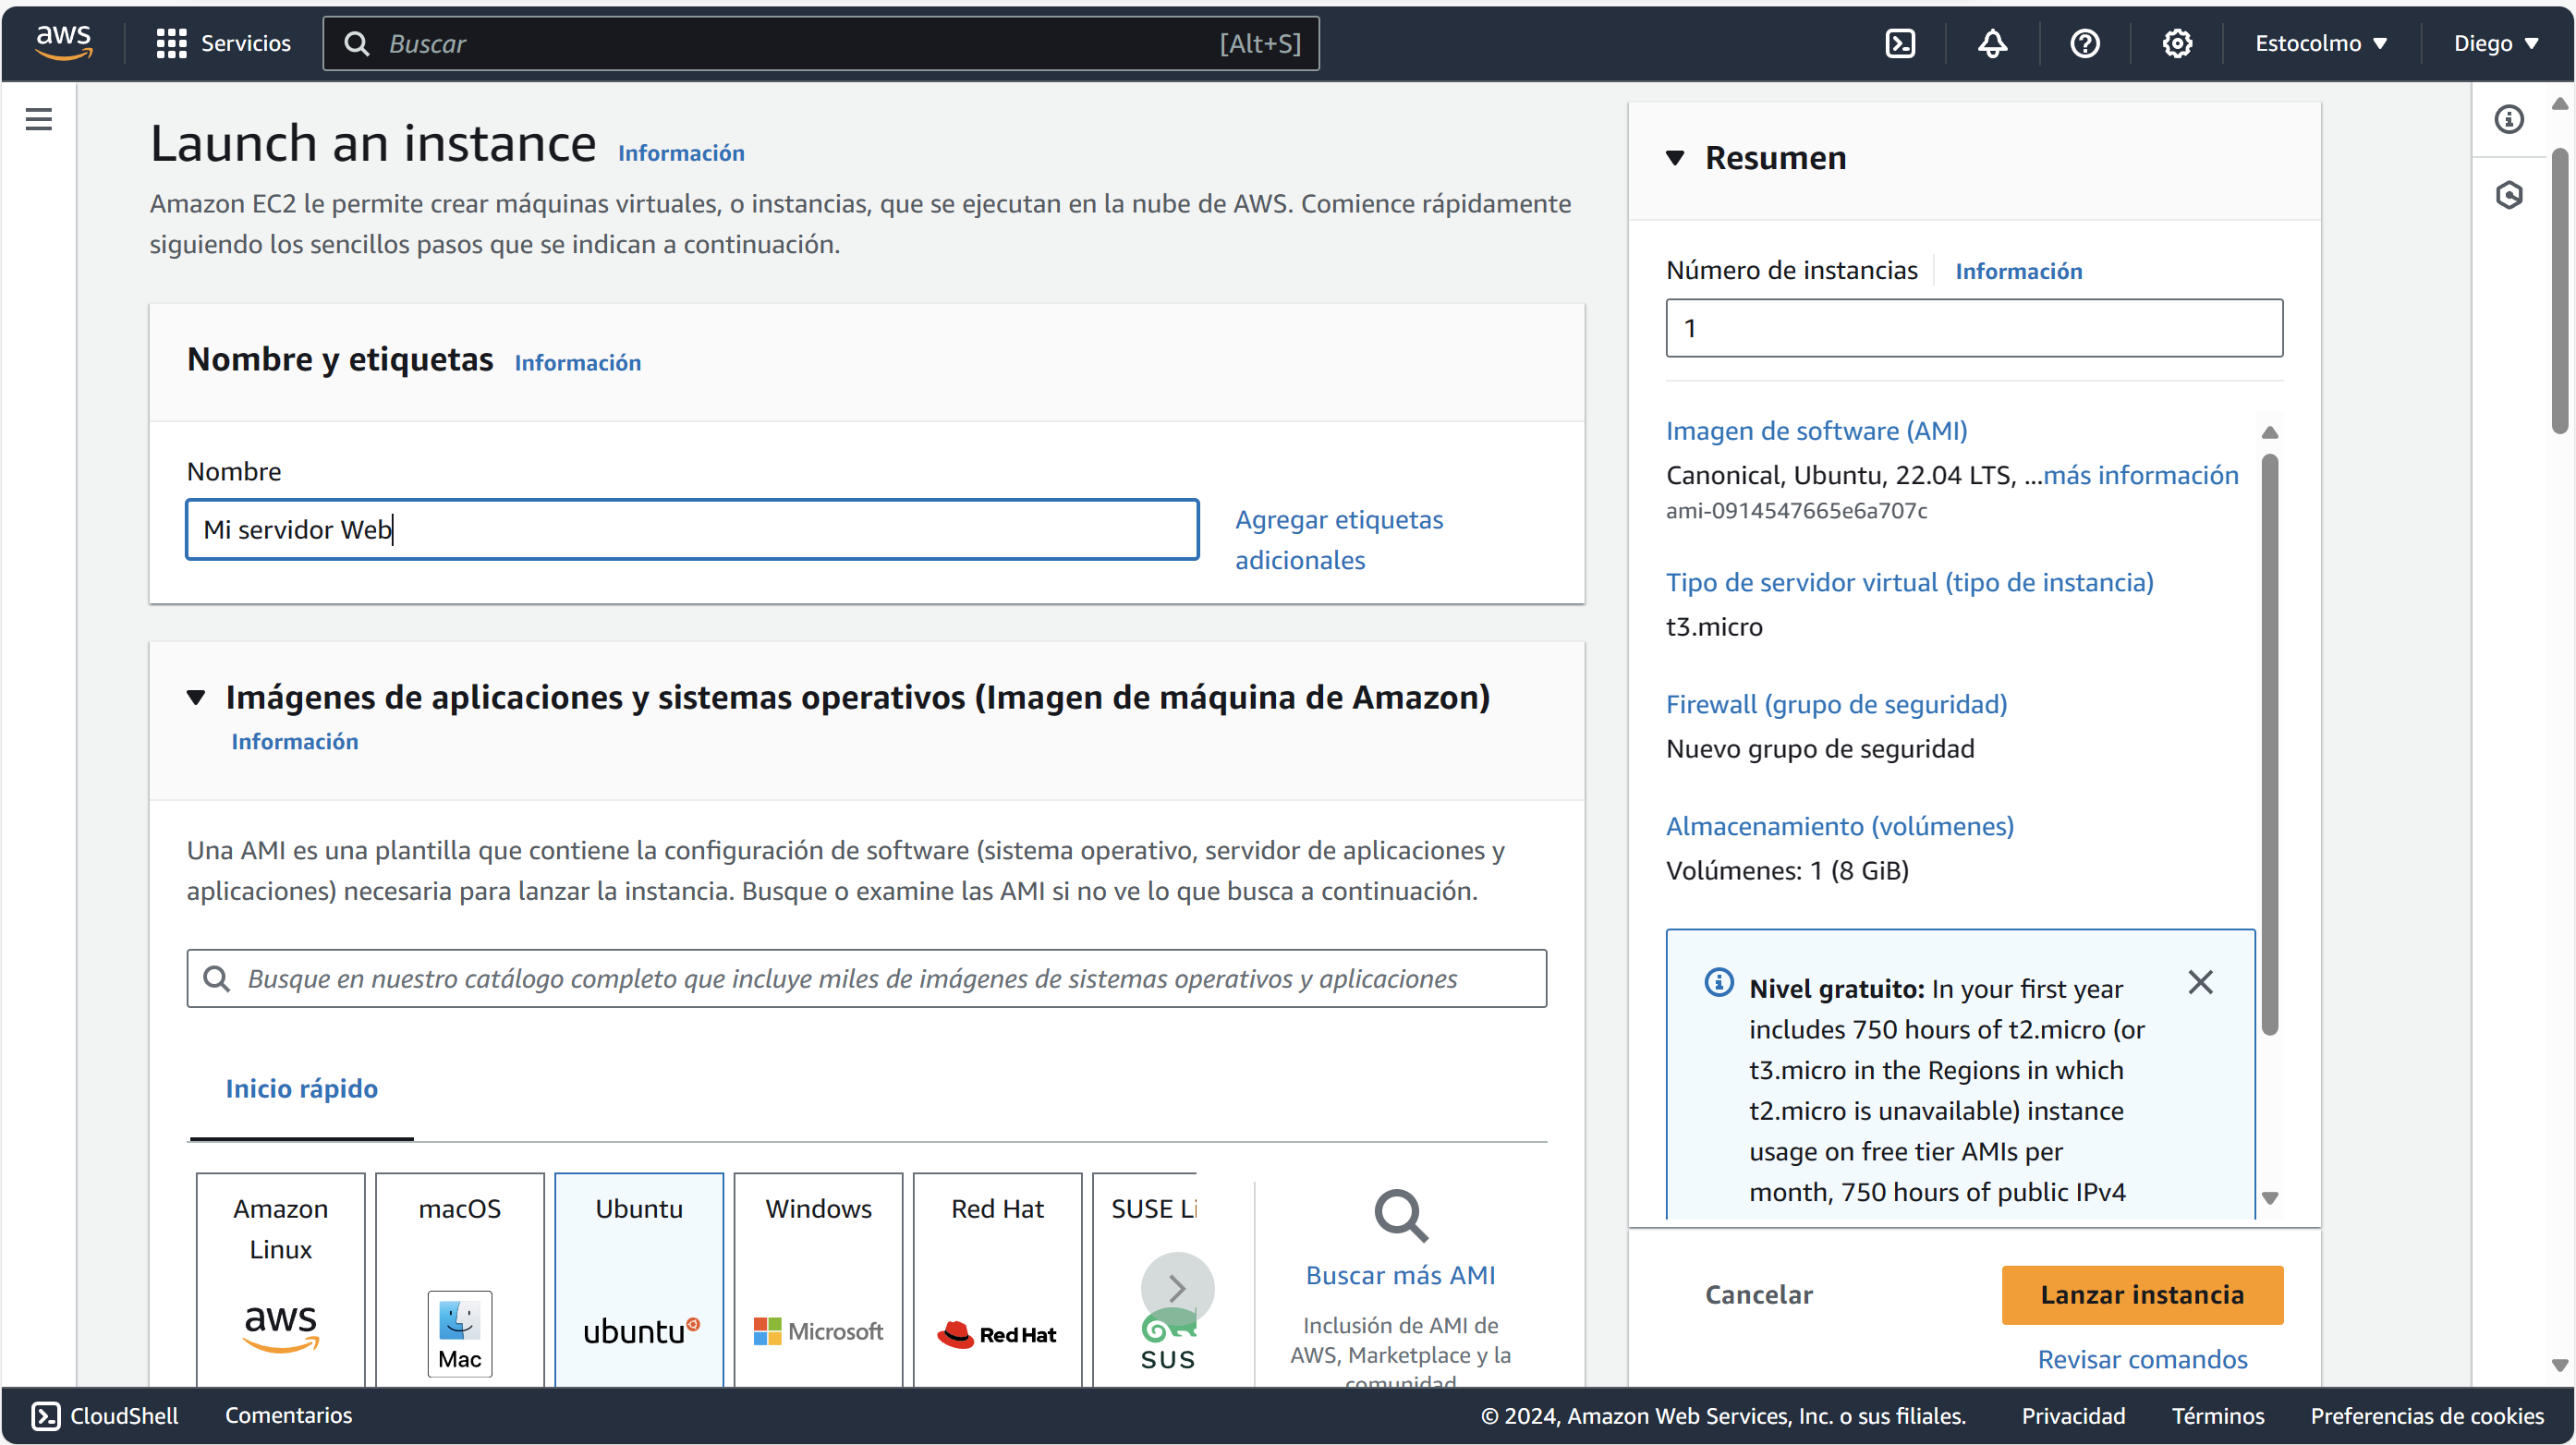
\includegraphics[width=0.5\linewidth]{Creacion_instancias.png}
    \caption{Creación del servidor web}
  \end{figure}

\newpage

% Seguridad y Configuración principal
\subsection{Securización y programación de script de mantenimiento}

% Cierre puertos en desuso
\subsubsection{Cerrar puertos de entrada y salida en desuso:}
\begin{enumerate}
    \item Identificar el ID del Grupo de Seguridad: \\
    \texttt{curl -s http://169.254.169.254/latest/meta-data/security-groups/}
    \item Revocar acceso a todos los puertos excepto el 22: \\
    \texttt{aws ec2 revoke-security-group-ingress --group-id tu-id-de-grupo --protocol all --cidr 0.0.0.0/0}
\end{enumerate}

\begin{figure}[ht]
    \centering
    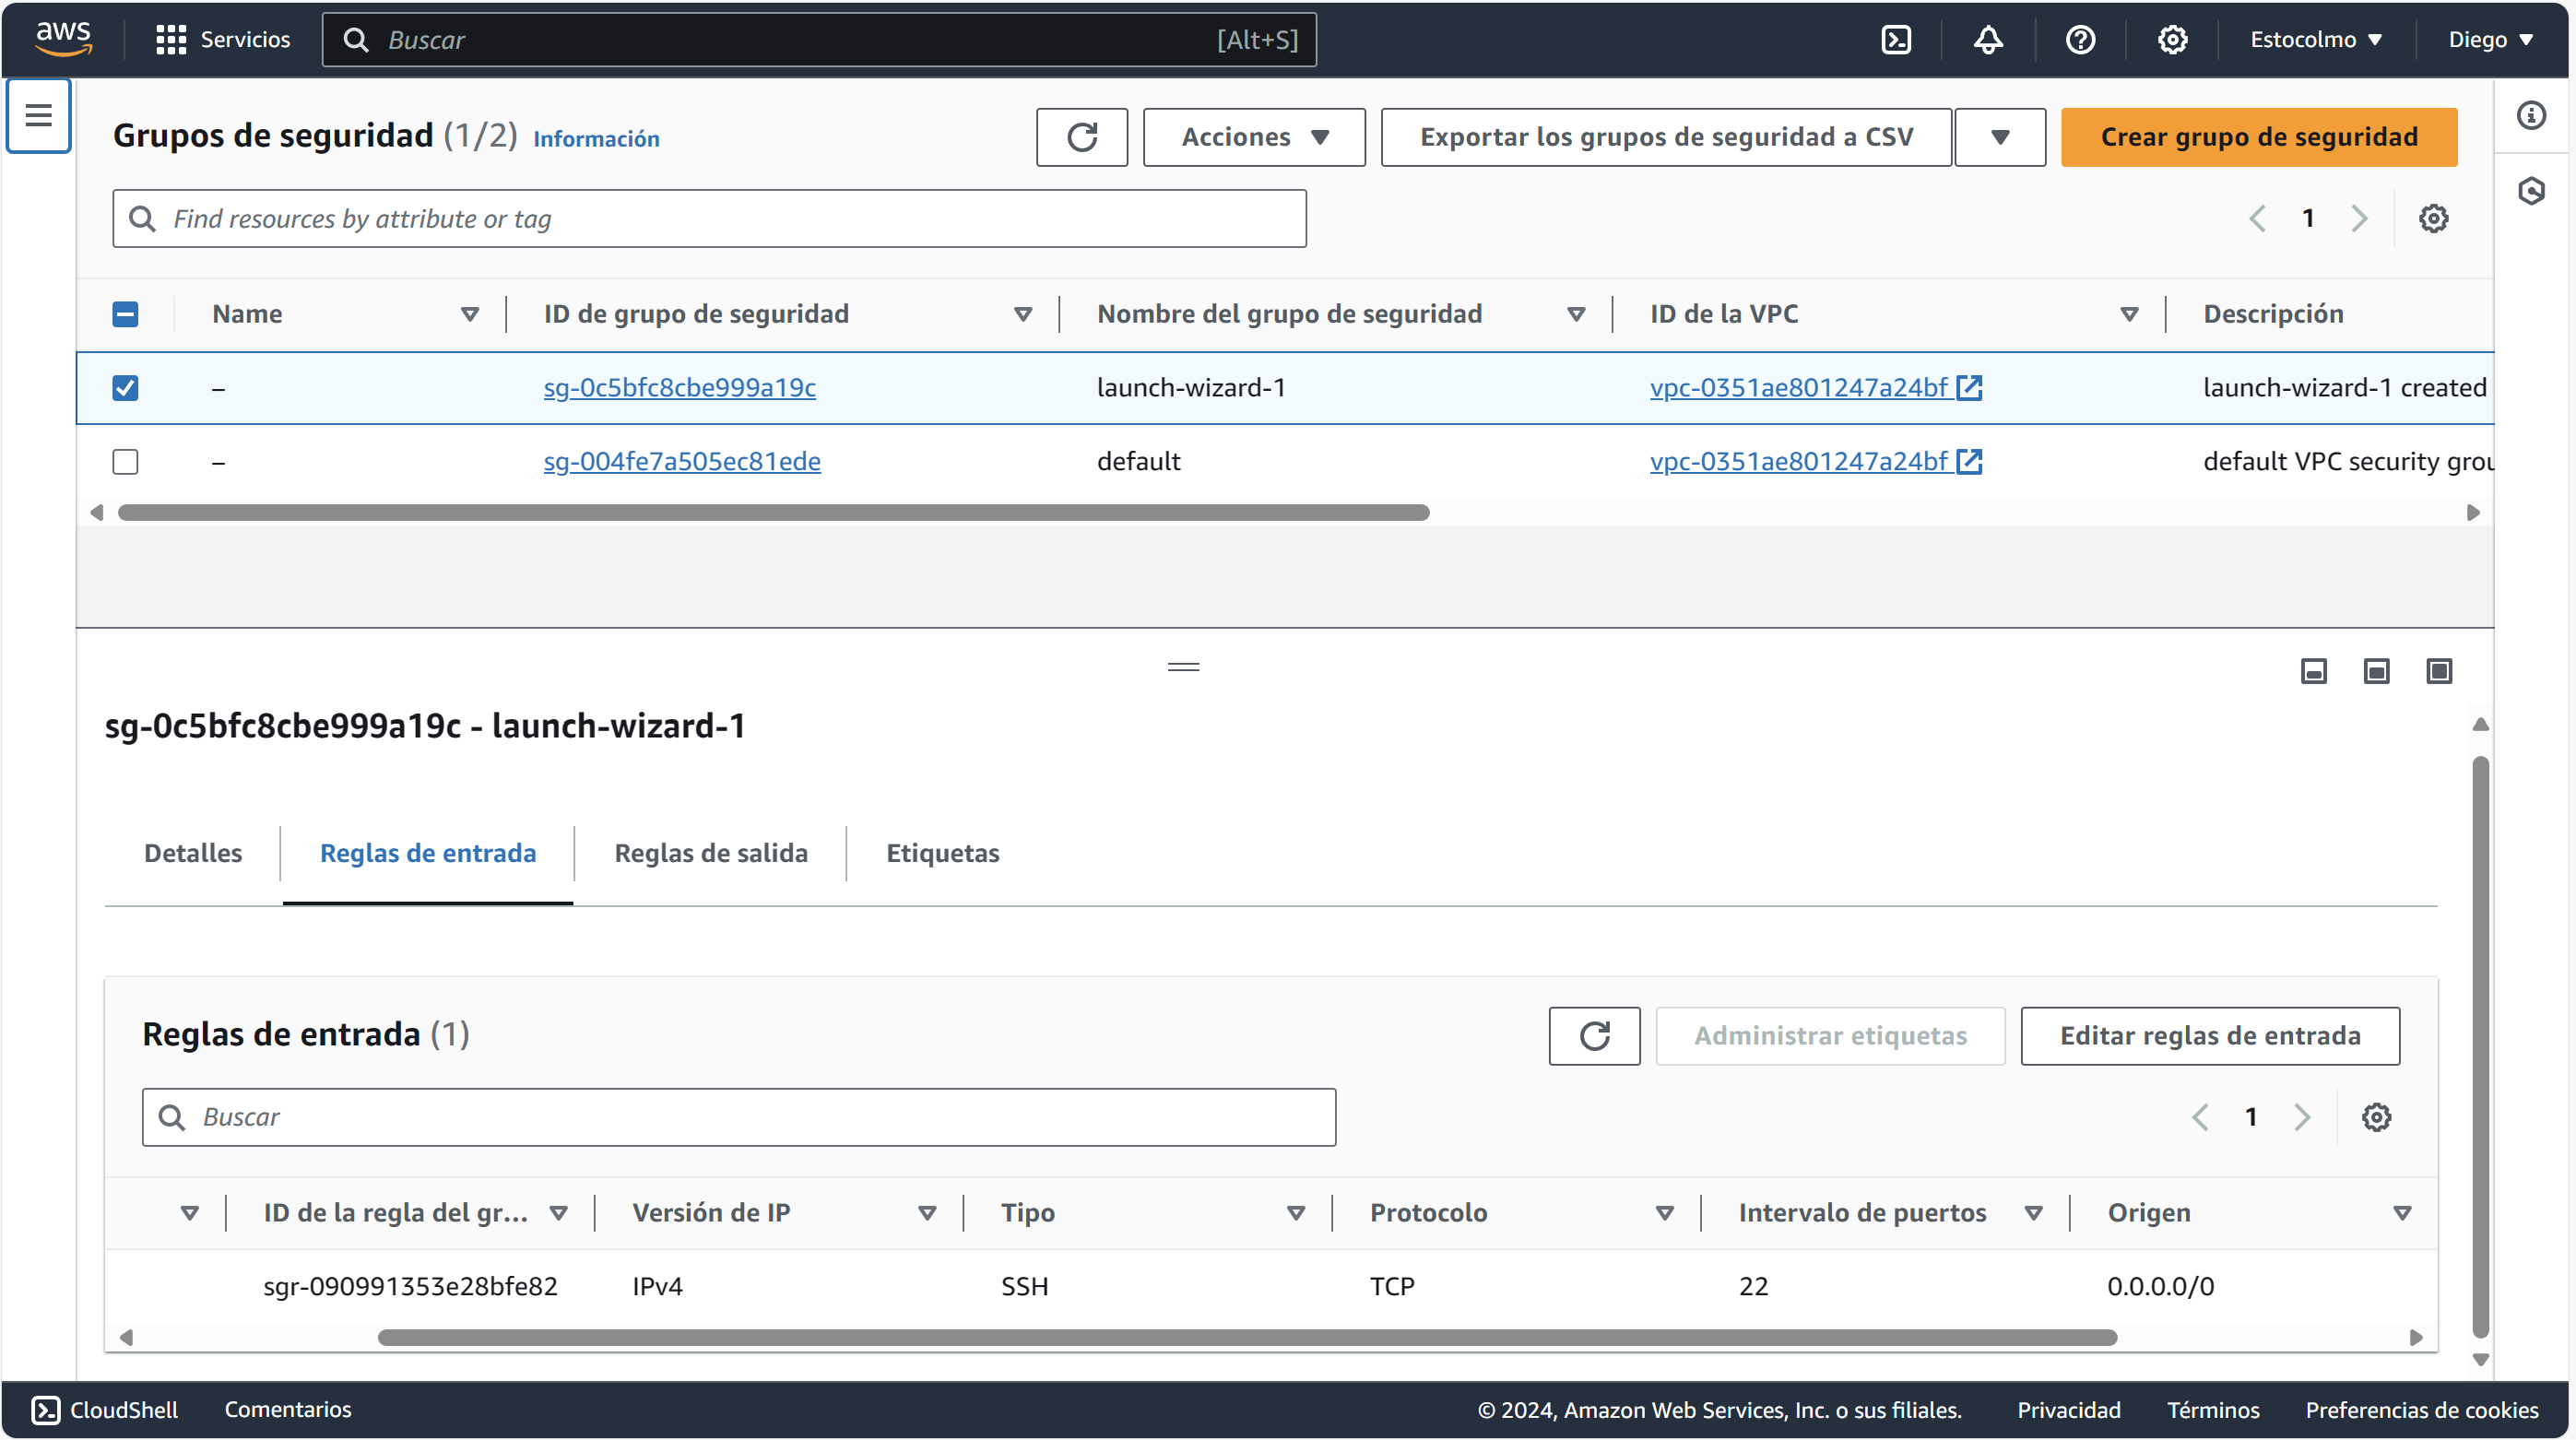
\includegraphics[width=0.5\linewidth]{Puertos_de_entrada.png}
    \caption{Configuración de Puertos de Entrada}
  \end{figure}

% Configuración programa seguridad
\subsubsection{Pasos para implementar Fail2ban:}
\begin{enumerate}
  \item Descargar Python (versión mayor o igual a 3.5)
  \item Actualizar el sistema: \texttt{sudo apt update}
  \item Instalar Python: \texttt{sudo apt install python3 python3-pip}
  \item Verificar la instalación: \texttt{pip3 --version}
  \item Ejecutar comando de instalación: \texttt{sudo apt install fail2ban}
  \item Configurar \textit{fail2ban} según los requisitos.
\end{enumerate}

% Script de mantenimiento
\subsubsection{Script de mantenimiento:}
\begin{lstlisting}[language=bash, caption=Script de mantenimiento]
#!/bin/bash

directorios_respaldar="/etc /var/lib /home/*"
directorio_backup="/home/directorio_backup"

fecha=$(date +"%Y-%m-%d")
tar_file="$directorio_backup/backup_$fecha.tar.gz"
tar -czvf "$tar_file" $directorios_respaldar

find /ruta/a/logs -type f -name "*.log" -mtime +7 -exec rm {} \;

echo "Copia de seguridad realizada en $tar_file"
echo "Archivos de log más antiguos de 7 días eliminados."
\end{lstlisting}

% Edición del Cron
\subsubsection{Automatización:}

Para automatizar la ejecución del script, modificar el cron con el comando: \texttt{crontab -e} \\
Agregar la siguiente línea al final del archivo: \\
\texttt{0 3 * * * /home/scripts/script\_backup.sh > /home/directorio\_backup/log\_backup.log 2>&1}

\

% API con Bottle
\subsection{Servicios}
\subsubsection{Crear la API mínima con Bottle}
\begin{enumerate}
  \item Instalar Bottle: \texttt{pip install bottle}
  \item Crear un archivo python que implemente los recursos requeridos.


\begin{lstlisting}[language=Python, caption=API básica con Bottle]
from bottle import Bottle, run
import datetime

app = Bottle()

@app.route('/hi')
def hello():
    now = datetime.datetime.now()
    return f'Hola, hoy es {now.strftime("%d/%m/%Y")} y son las {now.strftime("%H:%M:%S")}'

@app.route('/status')
def status():
    # Implementar lógica para listar servicios en ejecución
    return "Servicios en ejecución: Servicio1, Servicio2, ..."

if __name__ == '__main__':
    run(app, host='0.0.0.0', port=8080)
\end{lstlisting}

    \item Darle permisos de ejecución al archivo: \texttt{chmod +x /home/scripts/api.py}
    \item Permitir el acceso de tráfico entrante por el puerto 80 ejecutando:\\ \texttt{iptables -A INPUT -p tcp --dport 8080 -j ACCEPT}
    \item Redirigir el tráfico del puerto 8080 al puerto 80 (donde está la API):\\ \texttt{iptables -t nat -A PREROUTING -p tcp --dport 8080 -j REDIRECT --to-port 80}
    \item Crear el directorio iptables en /etc/: \texttt{sudo mkdir -p /etc/iptables/}
    \item Guardar las reglas de iptables: \texttt{sudo iptables-save > /etc/iptables/rules.v4}
\end{enumerate}


\newpage


% Supervisor
\subsection{Instalar y configurar Supervisor:}
\begin{enumerate}
    \item Ejecutar el siguiente comando: \texttt{sudo apt-get install supervisor}
    \item Crea un archivo de configuración para tu aplicación en Supervisor. \\ En este caso, api.conf en /etc/supervisor/conf.d/:
    \begin{lstlisting}[language=Python, caption=API básica con Bottle]
        [program:my_api]
        command=/usr/bin/python3 /home/scripts/api.py  # Ruta absoluta al script api.py
        directory=/home/scripts/  # Directorio donde se encuentra api.py
        autostart=true
        autorestart=true
        stderr_logfile=/var/log/api.err.log
        stdout_logfile=/var/log/api.out.log
        \end{lstlisting}
    \item Actualiza la configuración de Supervisor y comienza a supervisar tu aplicación:\\
        \texttt{sudo supervisorctl reread}\\ \texttt{sudo supervisorctl update}\\ \texttt{sudo supervisorctl start my\_api}
    \item Prueba de que la api funciona:
        \begin{enumerate}
            \item Prueba del programa hi: \texttt{curl http://localhost:8080/hi}
            \item Prueba del programa status: \texttt{curl http://localhost:8080/status}
        \end{enumerate}
\end{enumerate}


% Nginx y proxy inverso
\subsection{Instalar Nginx y configurar un proxy inverso:}
\begin{enumerate}
    \item Instalar Nginx: \texttt{sudo apt-get install nginx}
    \item Creamos un archivo de configuración para la API en Nginx. En nuestro caso, api.conf en /etc/nginx/sites-available/:
    \begin{lstlisting}[language=Python, caption=API básica con Bottle]
        server {
            listen 80;
            server_name tu_dominio_o_ip;

            location / {
                proxy_pass http://127.0.0.1:8080;  # Puerto donde se ejecuta la API con Bottle
                proxy_set_header Host $host;
                proxy_set_header X-Real-IP $remote_addr;
                proxy_set_header X-Forwarded-For $proxy_add_x_forwarded_for;
            }
        }
        \end{lstlisting}
    \item Habilitamos el sitio y reiniciamos Nginx:\\
        \texttt{sudo ln -s /etc/nginx/sites-available/api.conf /etc/nginx/sites-enabled/}\\ \texttt{sudo systemctl restart nginx}
\end{enumerate}


% Conclusión
\section{Conclusión}
En esta práctica, se han abordado de manera integral la configuración y administración básica de un servidor Linux, desde su creación en AWS hasta la implementación de medidas de seguridad como el cierre de puertos no utilizados y la configuración de Fail2ban. Además, se han automatizado tareas de mantenimiento mediante scripts y hemos desplegado una API-Rest utilizando Bottle, asegurándonos de su disponibilidad y seguridad con Supervisor y Nginx como proxy inverso. Estos pasos nos permiten tener un servidor funcional, seguro y con capacidades para gestionar servicios web de manera eficiente.


\end{document}
